\documentclass[a4paper]{article}
\usepackage[margin=0.52in]{geometry}
\usepackage{graphicx}

\begin{document}
\begin{LARGE}
       \begin{center}
         \textrm{\textbf{Sai Gopal Dhulipala}}
       \end{center} 
     \noindent\makebox[\linewidth]{\rule{\paperwidth}{0.4pt}}
\end{LARGE}
   \begin{Large}

     \begin{minipage}[t]{0.5\textwidth}
        Hostel No.10,\\
        Room No.B-486,\\
        NIT Kurukshetra,\\
        Haryana-136119.
     \end{minipage}
     \begin{minipage}[t]{0.5\textwidth}
        \textbf{Contact:} +91-9728433154\\
        \textbf{Email-id:} saigopaldhulipala@gmail.com
     \end{minipage}
   \end{Large}
   \begin{figure}[h]
         \begin{flushright}
           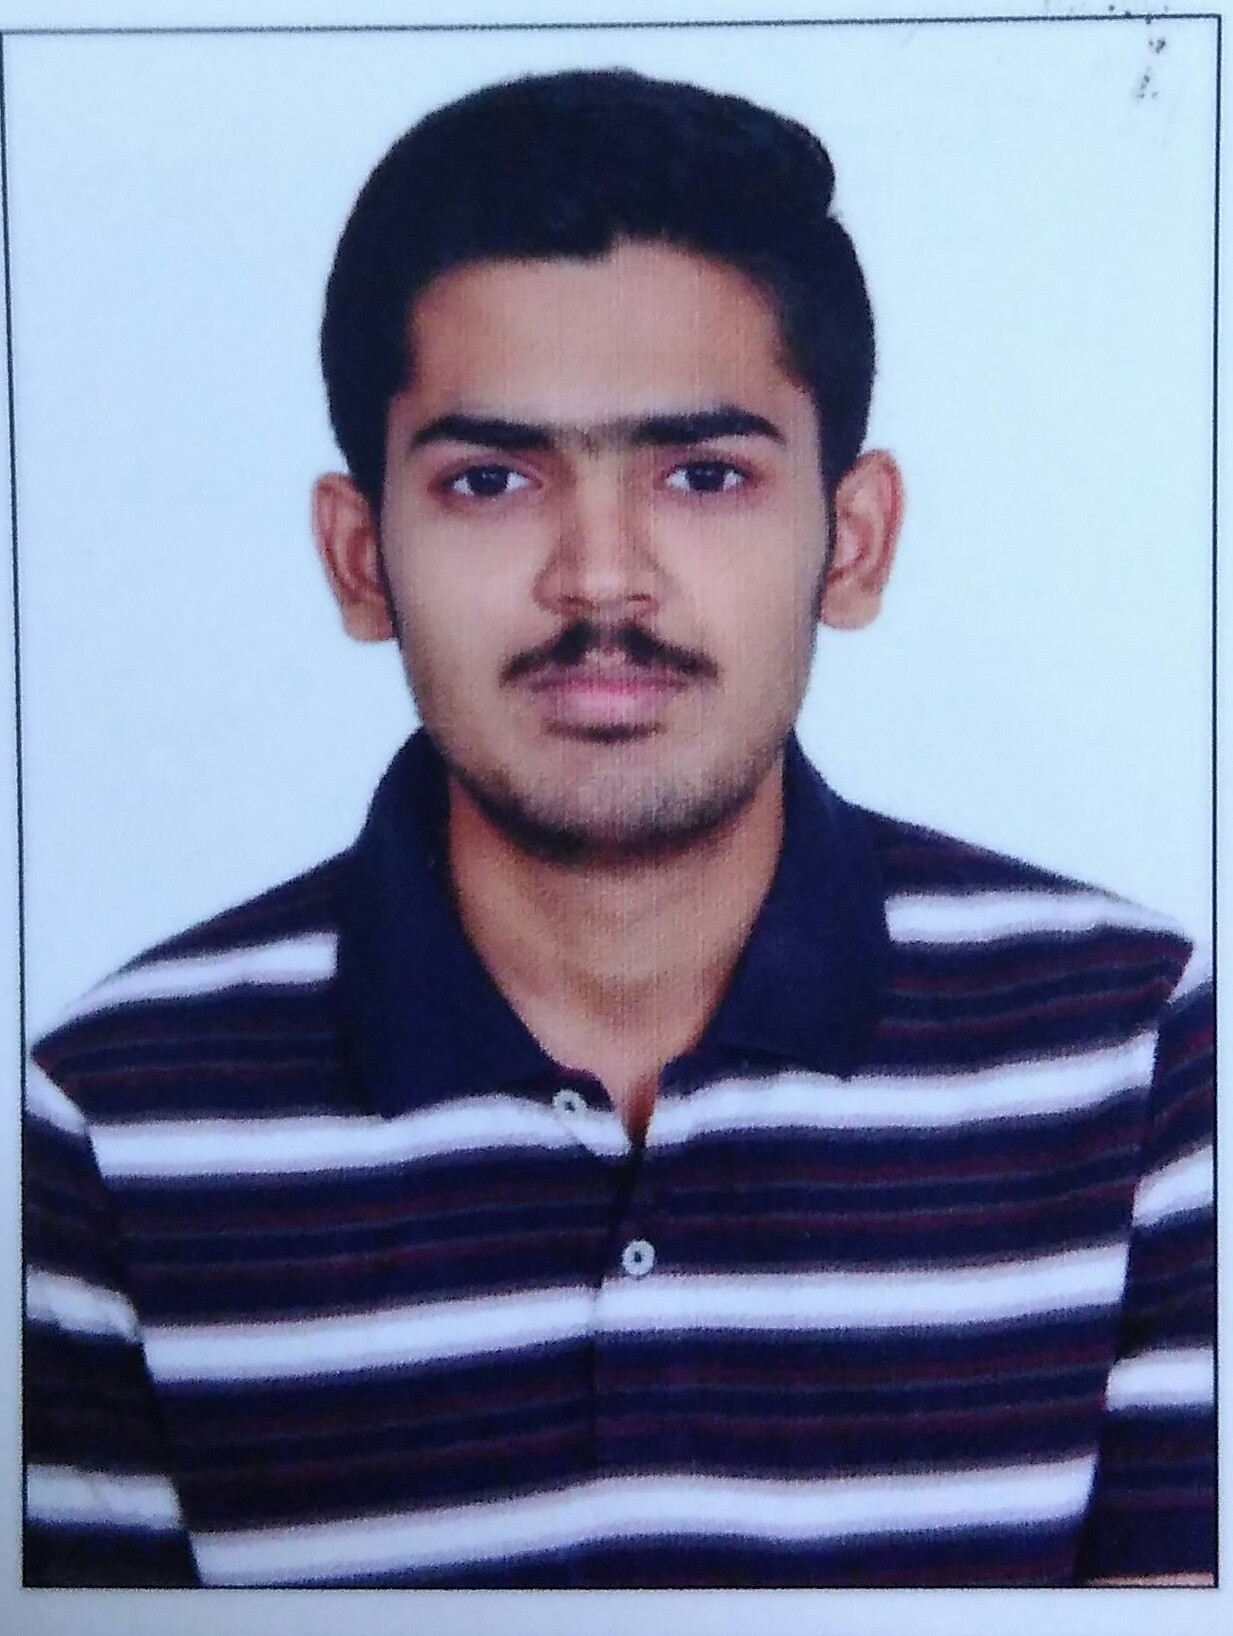
\includegraphics[width=3cm,height=4cm]{DSG.jpg}
         \end{flushright}
     \end{figure}
     \section*{\textbf{OBJECTIVE}}
Intend to work in tech environment which will help me to explore myself fully and realize my potential.Willing to work in challenging and creative environment.

\section*{\textbf{EDUCATION}}
\begin{table}[h]
\begin{tabular}{|c|c|c|c|}
\hline
\textbf{DEGREE} & \textbf{COLLEGE/SCHOOL} & \textbf{\begin{tabular}[c]{@{}c@{}}\\PASSING \\YEAR \end{tabular}} & \textbf{\begin{tabular}[c]{@{}c@{}}\\PASS \\ PERCENTAGE \end{tabular}} \\ \hline

\begin{tabular}[c]{@{}c@{}}\\Matriculation\\ (10th)\end{tabular} & Bhashyam Public, Rajahmundry, Andhra Pradesh & 2012 & 90.25\% \\ \hline

\begin{tabular}[c]{@{}c@{}}\\Intermediate\\ (11th, 12th)\end{tabular} & Sri Chaitanya College, Vijayawada, Andhra Pradesh & 2014 & 97.7\% \\ \hline

\begin{tabular}[c]{@{}c@{}}\\B.Tech\\ (Pursuing)\end{tabular} & NIT Kurukshetra, Haryana & 2018 & 8.2 (CGPA) \\ \hline
\end{tabular}
\end{table}

\section*{\textbf{PROJECTS}}
\begin{enumerate}
\item Created a \textbf{Smart Garbage Monitoring System} which has WiFi connectivity, Bluetooth connectivity, an RFID Reader unit, garbage level monitoring unit, a display unit, an automatic mouth opening and closing system. Also created an Android app which shows the status of all the bins in the city. Participated and got first position in national level event ``Micrologic" during
Techfest at NIT Kurukshetra
\item \textbf{Wireless land rover} with a robotic arm (used 3-axis Accelerometer ADXL335 for robot movement and RF module for wireless communication between remote and robot). Participated and got second position in  national level event ``Roborynth" during Techfest at NIT Kurukshetra. The problem statement of the competitions was to design a wireless remote control robot that can pick and place the objects.
\item \begin{flushleft} Participated and got second position in \textbf{``Launch a module"} theme of e-yantra robotics competition 2016 conducted by IIT Bombay.\end{flushleft} 
\end{enumerate}

\section*{\textbf{TRAINING}}
\begin{itemize}
\item Did 6 weeks Summer training (8th June'16 - 21st July'16) on NXP's (founded by Philips) LPC2148 ARM7 based 32-bit RISC Microcontroller, Atmel AT89S52 CMOS 8-bit Microcontroller and Wireless communication modules.  
\end{itemize}

\section*{\textbf{TECHNICAL SKILLS}}
\begin{itemize}
\item \textbf{Embedded controllers and Processors:}
   \begin{itemize}
      \item AT89x51, AT89x52
      \item ARM architecture based LPC2148
      \item Atmega 2560
      \item 8086 Microprocessor
   \end{itemize}
\item \textbf{Embedded IDE:} Atmel studio, KEIL 
\item \textbf{EDA Tools:} Orcad, Proteus, Model Sim
\item \textbf{Languages:} Embedded C, Assembly(8086), VHDL(basics), C, C++(basics)
\end{itemize}

\section*{\textbf{SOFT SKILLS}}
\begin{enumerate}
\item Positive Attitude
\item Adaptable
\item Determined
\item Self-Confident
\end{enumerate}

\section*{\textbf{EXTRA CIRRICULAR ACTIVITIES}}
\begin{itemize}
\item A member of club SHIKSHA, Student Society for Social Action in NIT Kurukshetra, which holds regular classes throughout the year to assist students in fulfilling their academic goals. 
\item Bicycling
\end{itemize}

\section*{\textbf{Co-CIRRICULAR ACTIVITIES}}
\begin{enumerate}
\item Participate frequently in athletic activities conducted at our college.
\item Participated in marathon runs and bicycling events  conducted by various teams under various campaigns at our college.
\end{enumerate}

\section*{\textbf{PERSONAL INFORMATION}}
Father's Name  : Phani Kumar Dhulipala\\
Mother's Name  : Padmaja Dhulipala\\
Sex            : Male\\
Date of Birth  : 5th February, 1997\\
Nationality    : Indian\\
Marital Status : Single

\section*{\textbf{LANGUAGES KNOWN}}
Telugu, Hindi, English

\section*{\textbf{REFERENCE}}
\begin{enumerate}
\item Dr.Rajoo Pandey,\\
Head of Department,\\
ECE Department,\\
NIT Kurukshetra,\\
email-id: rtatnitk@gmail.com\\
Phone No. : +91-9416840435
\item Mr.Trailokya Nath Sasamal,\\
Assistant Professor,\\
ECE Department,\\
NIT Kurukshetra,\\
Phone No. : +91-8950333079
\end{enumerate}

\section*{\textbf{DECLARATION}}
I hereby declare that the above information is accurate to the best of my knowledge.\\
---Sai Gopal
\end{document}
